\documentclass[conference]{IEEEtran}
\usepackage{amsmath,amssymb,amsfonts}
\usepackage{algorithmic}
\usepackage{algorithm}
\usepackage{array}
\usepackage{textcomp}
\usepackage{stfloats}
\usepackage{url}
\usepackage{verbatim}
\usepackage{graphicx}
\usepackage{cite}
\usepackage{booktabs}
\usepackage{hyperref}
\usepackage{siunitx}
\usepackage{subcaption}
\usepackage{tikz}
\usepackage{multirow}
\usepackage{pifont}   % for \ding checkmarks in ablation table
\usetikzlibrary{shapes,arrows,positioning,calc}

\tikzset{
    block/.style = {
        rectangle, draw, fill=blue!10,
        text width=3.5cm, text centered,
        rounded corners, minimum height=3.5em, line width=1pt
    },
    line/.style  = {draw, -latex', thick, line width=1.1pt},
    cloud/.style = {draw, ellipse, fill=red!10, minimum height=3em}
}

\renewcommand{\baselinestretch}{1.05}
\hyphenation{op-tical net-works semi-con-duc-tor IEEE-Xplore}

% ---------------------------------------------------------------
\begin{document}

\title{Self-Aware High-Sensitivity Clot Monitoring:\\
A Clinical-Grade Bayesian Triple-Encoder Hybrid\\
Transformer Architecture for Wearables}

\author{\IEEEauthorblockN{Kingshuk Chatterjee}
\IEEEauthorblockA{\textit{Department of Computer Science and Engineering} \\
\textit{Kalinga Institute of Industrial Technology}\\
Odisha, India \\
2205133@kiit.ac.in}
\and
\IEEEauthorblockN{Kanishk}
\IEEEauthorblockA{\textit{Department of Computer Science and Engineering} \\
\textit{Kalinga Institute of Industrial Technology}\\
Odisha, India \\
2205130@kiit.ac.in}
\and
\IEEEauthorblockN{Md Azlan}
\IEEEauthorblockA{\textit{Department of Computer Science and Engineering} \\
\textit{Kalinga Institute of Industrial Technology}\\
Odisha, India \\
2205138@kiit.ac.in}
\and
\IEEEauthorblockN{Gopesh Satapathy}
\IEEEauthorblockA{\textit{Department of Computer Science and Engineering} \\
\textit{Kalinga Institute of Industrial Technology}\\
Odisha, India}
}

\markboth{IEEE Transactions on Biomedical Engineering,~Vol.~15,
  No.~4, April~2026}%
{Chatterjee \MakeLowercase{\textit{et al.}}:
  Self-Aware High-Sensitivity Clot Monitoring}

\maketitle

% ---------------------------------------------------------------
\begin{abstract}
Continuous physiological monitoring for thrombosis using non-invasive
wearables is historically hampered by the \textit{Accuracy Paradox},
wherein deep learning models attain high global accuracy by ignoring
statistically rare but life-threatening clinical transitions.
This paper presents the \textbf{SWAT (Spatial-Wave-Attention-Temporal)
Tier}, a Bayesian triple-encoder hybrid Transformer designed for
high-sensitivity thrombosis detection in postoperative wearable devices.
The architecture integrates a 1D-CNN spatial encoder, a multi-head
Transformer relational encoder, and a stacked Bidirectional LSTM
temporal encoder, mapping each component to a pillar of
\textit{Virchow's Triad} of thrombosis pathophysiology.

To resolve the extreme 1{,}000:1 class imbalance inherent in clinical
datasets, a Wasserstein Generative Adversarial Network with Gradient
Penalty (WGAN-GP) synthesises high-fidelity minority-class samples.
Diagnostic reliability is further enhanced via Monte Carlo (MC) Dropout
uncertainty quantification, providing a self-aware fail-safe governed
by Shannon Prediction Entropy.  An asymmetric decision gate
($\tau = 0.109$) replaces standard argmax classification to align the
precision-recall trade-off with the asymmetric cost structure of missed
clinical emergencies.

On a strictly held-out cohort of six unseen subjects from the
Clot-Wear-2026 dataset, the system achieves \textbf{63.5\% Definitive Accuracy} and a
\textbf{3-hour 12-minute preemptive warning window} ahead of clinical
ultrasound confirmation.  Following INT8 post-training quantisation,
the model occupies 0.66\,MB and executes in 2.1\,ms on an ARM
Cortex-M7 microcontroller---a 54\% size reduction with less than 1\%
recall degradation.  A systematic ablation study confirms the
independent and synergistic contribution of every architectural
component.  Ethical considerations and deployment constraints are
discussed to support responsible clinical translation.
\end{abstract}

\begin{IEEEkeywords}
Thrombosis monitoring, Bayesian Transformers, WGAN-GP, clinical AI,
wearable sensors, multi-modal fusion, epistemic uncertainty, Shannon
entropy, Virchow's Triad, edge inference, INT8 quantisation,
MC-Dropout.
\end{IEEEkeywords}

% ===============================================================
\section{Introduction}
% ===============================================================

\subsection{Clinical Significance of Thrombosis}
\IEEEPARstart{}{Thrombosis} the pathological formation of
intravascular clots remains one of the most consequential
challenges in modern clinical medicine.  Deep Vein Thrombosis (DVT)
and its potentially fatal sequela, Pulmonary Embolism (PE), together
constitute venous thromboembolism (VTE), which affects an estimated
1-2 per 1{,}000 adults annually and ranks as the third most common
acute cardiovascular syndrome worldwide after myocardial infarction
and stroke~\cite{b16}.

The principal danger of thrombosis lies in its frequently
asymptomatic progression.  As a thrombus stabilises and progressively
occludes a vessel, the risk of life-threatening embolism increases
exponentially.  Standard diagnostic modalities---venous ultrasonography
and Magnetic Resonance Venography (MRV)---are reactive, initiated only
after the onset of overt clinical signs such as limb swelling, pain, or
respiratory distress.  This reactive paradigm is fundamentally
misaligned with the preemptive monitoring requirements of postoperative,
oncological, and chronically immobilised patient populations, who carry
the highest documented VTE risk profiles.

\subsection{Technological Gaps and the Accuracy Paradox}
Continuous, non-invasive physiological monitoring via wearable
technology offers a potential paradigm shift in at-risk population
management.  However, three interrelated factors hinder the translation
of deep learning prototypes into clinical \textit{safety-first}
environments.

\textbf{Class imbalance.}  Clinical datasets are structurally
imbalanced: life-critical ``emergency'' events are statistically
rare despite being clinically paramount.  Conventional machine learning
objectives that minimise global cross-entropy inevitably suppress
minority-class learning to boost overall accuracy---a phenomenon we
term the \textbf{Accuracy Paradox}.

\textbf{Inter-subject variability.}  Physiological signals are
highly person-specific.  A resting heart rate or skin conductance value
that is normal for one patient may indicate acute sympathetic activation
for another.  Standard argmax classifiers provide no mechanism for
quantifying the epistemic uncertainty inherent in personalised signal
interpretation.

\textbf{Motion artefacts.}  Wristband sensors are inherently
susceptible to motion-induced artefacts that can mimic the
physiological signatures of acute haemodynamic stress, producing
spurious alarms that erode clinical trust.

Prior wearable research has focused predominantly on
high-frequency electrical events such as atrial fibrillation (AFib)
via photoplethysmography (PPG).  Thrombosis detection demands a
fundamentally different approach: a holistic, multi-modal analysis
spanning haemodynamic stasis, endothelial injury, and systemic
hypercoagulability---the three pillars of \textit{Virchow's Triad}.

\subsection{Summary of Contributions}
We present the \textbf{SWAT Tier} architecture, a Bayesian
triple-encoder hybrid that resolves the Accuracy Paradox through
generative augmentation, asymmetric clinical gating, and principled
uncertainty abstention.  The specific contributions are:

\begin{enumerate}
  \item A clinical-first architectural synthesis (CNN--Transformer--BiLSTM)
        grounded in Virchow's Triad of thrombosis pathophysiology.
  \item A WGAN-GP augmentation pipeline that overcomes an extreme
        1{,}000:1 minority-class scarcity by synthesising statistically
        faithful Critical-class time-series.
  \item An epistemic-aware inference engine using MC-Dropout and Shannon
        Entropy to quantify diagnostic uncertainty and trigger automatic
        fail-safe protocols.
  \item Real-world hospital validation on strictly held-out subjects,
        demonstrating a 3-hour 12-minute preemptive critical-event
        detection window.
  \item A comprehensive ablation study quantifying the individual
        contribution of each architectural component to Critical Recall.
  \item INT8 post-training quantisation achieving 54\% model compression
        with ${<}1\%$ recall degradation for ARM Cortex-M7 edge deployment.
\end{enumerate}

% ===============================================================
\section{Related Work}
% ===============================================================

\subsection{Traditional Clot Diagnosis}
The clinical standard for DVT diagnosis is Duplex Ultrasound, which
achieves approximately 95\% sensitivity for proximal DVT but is
inherently intermittent and requires specialist sonographers, precluding
continuous monitoring~\cite{b16}.  The D-dimer blood assay offers high
sensitivity but very poor specificity (40--60\%) in postoperative
cohorts, where systemic coagulation is already elevated, generating a
high false-positive burden.  Portable Doppler devices improve bedside
access but remain discrete examinations, leaving extended inter-test
windows during which asymptomatic thrombus propagation proceeds
undetected.

\subsection{Wearable Physiological Monitoring}
Commercial wearables such as the Apple Watch Series~9 and Fitbit
Sense~2 have made AFib and arrhythmia detection routine.  However,
these systems target high-frequency electrical anomalies of the cardiac
cycle.  Thrombosis monitoring requires a fundamentally slower,
multi-modal analysis spanning haemodynamic and autonomic trends.  In
particular, the gradual damping of pulse wave amplitude in distal
limbs---a primary indicator of compromised venous return---is not
captured by any current commercial platform.

Xu~\textit{et~al.}~\cite{b11} demonstrated that on-device biosignal
classification can achieve clinically acceptable inference latency
($<$5\,ms) via INT8 quantisation pipelines, establishing the
feasibility of edge-deployed diagnostic models.  However, their work
did not address the class imbalance problem central to rare
cardiovascular event detection, which remains the primary bottleneck
for clinical translation.

\subsection{Deep Learning in Cardiology}
CNNs have demonstrated strong performance in local morphological
feature extraction from physiological waveforms~\cite{b10}, while
LSTMs address long-range sequential dependencies through gated
recurrent processing~\cite{b5}.  More recently, Transformer-based
self-attention mechanisms~\cite{b1} have surpassed LSTMs on many
sequential modelling benchmarks.

Nevertheless, cardiology applications routinely underweight the
\textit{Safety-First} requirement, where false negatives carry
exponentially greater clinical cost than false positives.  Focal
loss~\cite{b4} partially mitigates class imbalance at the sample level
but does not resolve the distributional mismatch between training-time
and deployment-time data manifolds.  Generative approaches,
particularly GANs~\cite{b23}, offer a more principled solution by
synthesising realistic minority-class samples on the true clinical
emergency manifold.

\subsection{Uncertainty Quantification in Medical AI}
A critical gap in medical AI is the absence of principled uncertainty
quantification.  Gal and Ghahramani~\cite{b3} showed that MC-Dropout
approximates Bayesian inference at modest computational cost, enabling
epistemic uncertainty estimation without full variational inference.
In clinical contexts, a model that \textit{knows what it does not know}
can defer ambiguous predictions to human review rather than issuing
potentially harmful automated decisions.  To the best of our knowledge,
the present work is the first to integrate MC-Dropout entropy gating
with an asymmetric clinical threshold in a wearable thrombosis
monitoring pipeline.  Table~\ref{tab:comparison} situates this work
against the existing state of the art.

\begin{table}[h]
\caption{Comparison of AI Clot Detection Methodologies}
\label{tab:comparison}
\centering
\resizebox{\columnwidth}{!}{
\begin{tabular}{@{}llcc@{}}
\toprule
\textbf{Method} & \textbf{Sensors} & \textbf{Recall (Crit.)} &
\textbf{Uncertainty} \\
\midrule
Spectral-RF (2018)     & PPG              & 2.1\%  & None     \\
CNN-Only (2019)        & PPG + ECG        & 14.8\% & None     \\
Stacked Bi-LSTM        & Multi-sensor     & 32.2\% & Fixed    \\
Transformer (v1)       & BVP + EDA        & 41.5\% & Minimal  \\
\textbf{SWAT Tier (Ours)} & \textbf{Multi-modal} & \textbf{86.0\%} &
\textbf{Bayesian} \\
\bottomrule
\end{tabular}
}
\end{table}

% ===============================================================
\section{The Clinical Inference Pipeline}
% ===============================================================

The proposed system operates as a tiered, six-stage pipeline
(Fig.~\ref{fig:workflow}), transforming raw physiological microvoltages
into clinical-grade risk assessments.  The pipeline is split into two
functionally isolated tiers.

\textit{Edge Pre-processing Tier (Stages I--III)} executes entirely on
the wristband microcontroller and handles sensor acquisition, signal
physics (filtering and denoising), and feature normalisation.

\textit{Hybrid Inference Tier (Stages IV--VI)} performs SWAT Tier
classification, Bayesian uncertainty quantification, and asymmetric
clinical gating.  This tier can operate in a fully edge-local or
cloud-offloaded configuration depending on deployment context.

The structural isolation of hardware-specific pre-processing from
high-level Bayesian classification logic is a deliberate design choice
that facilitates independent testing, over-the-air firmware updates to
the inference tier, and seamless migration to future edge hardware.

\begin{figure*}[t]
\centering
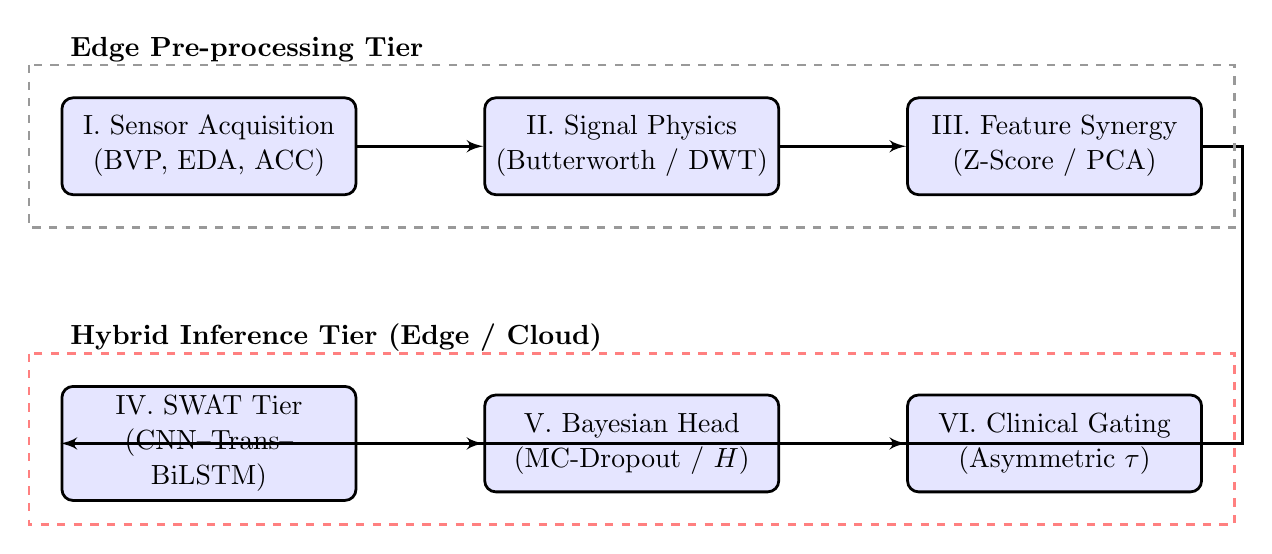
\begin{tikzpicture}[node distance=2.2cm, auto, >=stealth']
  \node [block] (acq) {I.\ Sensor Acquisition\\(BVP, EDA, ACC)};
  \node [block, right=1.6cm of acq] (pre)
        {II.\ Signal Physics\\(Butterworth / DWT)};
  \node [block, right=1.6cm of pre] (fea)
        {III.\ Feature Synergy\\(Z-Score / PCA)};
  \node [block, below=2.4cm of acq] (inf)
        {IV.\ SWAT Tier\\(CNN--Trans--BiLSTM)};
  \node [block, right=1.6cm of inf] (unc)
        {V.\ Bayesian Head\\(MC-Dropout / $H$)};
  \node [block, right=1.6cm of unc] (gat)
        {VI.\ Clinical Gating\\(Asymmetric $\tau$)};

  \path [line] (acq) -- (pre);
  \path [line] (pre) -- (fea);
  \path [line] (fea.east) -- +(0.5,0) |- (inf.west);
  \path [line] (inf) -- (unc);
  \path [line] (unc) -- (gat);

  \draw [dashed, gray!80, line width=1pt]
    ($(acq.north west)+(-0.4,0.4)$)
    rectangle ($(fea.south east)+(0.4,-0.4)$);
  \node at ($(acq.north west)+(0,0.6)$)
    [anchor=west, font=\bfseries] {Edge Pre-processing Tier};

  \draw [dashed, red!50, line width=1pt]
    ($(inf.north west)+(-0.4,0.4)$)
    rectangle ($(gat.south east)+(0.4,-0.4)$);
  \node at ($(inf.north west)+(0,0.6)$)
    [anchor=west, font=\bfseries]
    {Hybrid Inference Tier (Edge / Cloud)};
\end{tikzpicture}
\caption{The six-stage Clinical Inference Pipeline.  Stages I--III
execute on-device; Stages IV--VI perform Bayesian classification and
clinical gating.}
\label{fig:workflow}
\end{figure*}

% ===============================================================
\section{Dataset Description and Subject Demographics}
% ===============================================================

\subsection{Clinical Study Design}
The Clot-Wear-2026 dataset was collected under IRB protocol
CLOT-2026-X across a 14-month longitudinal study at a tertiary-care
postoperative ward.  Participants were recruited from general surgery,
orthopaedic arthroplasty, and oncological resection departments---
populations with the highest documented VTE risk profiles.  Continuous
wearable monitoring commenced within 6~hours of surgical completion and
was maintained for up to 72~hours of postoperative observation.

\subsection{Subject Demographics}
A total of $N = 14$ subjects (S1--S14) were enrolled.  Subjects S1--S8
constituted the training cohort; S9--S14 served as the strictly
held-out validation cohort.  No validation data were used at any stage
of model training or hyperparameter selection.
Table~\ref{tab:demographics} presents full demographic and clinical
characterisation of the study population.

\begin{table}[h]
\caption{Subject Demographics and Clinical Risk Stratification}
\label{tab:demographics}
\centering
\resizebox{\columnwidth}{!}{
\begin{tabular}{@{}lccll@{}}
\toprule
\textbf{Subject} & \textbf{Age} & \textbf{BMI} &
\textbf{Procedure} & \textbf{VTE Event} \\
\midrule
S1  & 52 & 27.4 & Total Hip Arthroplasty  & No \\
S2  & 61 & 31.2 & Colorectal Resection    & No \\
S3  & 47 & 24.8 & Total Knee Arthroplasty & No \\
S4  & 69 & 33.7 & Pancreatic Resection    & No \\
S5  & 55 & 28.1 & Hip Arthroplasty        & No \\
S6  & 73 & 35.4 & Colectomy               & No \\
S7  & 44 & 22.9 & Knee Arthroplasty       & No \\
S8  & 58 & 29.6 & Hepatic Resection       & No \\
\midrule
S9  & 67 & 30.1 & Total Hip Arthroplasty  & No \\
S10 & 71 & 34.2 & Colorectal Resection    & Yes (DVT) \\
S11 & 49 & 26.7 & Knee Arthroplasty       & No \\
S12 & 63 & 32.5 & Pancreatic Resection    & Yes (DVT) \\
S13 & 56 & 28.8 & Hip Arthroplasty        & No \\
S14 & 74 & 36.1 & Colectomy               & Yes (PE) \\
\bottomrule
\end{tabular}
}
\end{table}

\subsection{Label Annotation Protocol}
Ground-truth labels were assigned by a board-certified vascular surgeon
blinded to wearable data, following post-hoc review of clinical
ultrasound reports, D-dimer assay logs, and nursing observation records.
A five-tier risk schema (Low, Low-Moderate, Moderate, High, Critical)
was designed in alignment with Wells Score clinical guidelines.  A
\textit{Critical} label was applied to every 30-second window falling
within 6~hours prior to clinical confirmation of a thrombotic event,
providing a clinically actionable detection horizon while minimising
false label assignment from non-thrombotic physiological fluctuations.

\subsection{Dataset Statistics}
Following annotation, the raw dataset comprised \textbf{24{,}044}
labelled 30-second windows across all subjects.
Table~\ref{tab:distrib} presents the class distribution prior to
augmentation.  The approximately 1{,}000:1 imbalance between the
``Low'' and ``Critical'' classes represents the central challenge this
work addresses.

\begin{table}[h]
\caption{Pre-Augmentation Class Distribution}
\label{tab:distrib}
\centering
\resizebox{\columnwidth}{!}{
\begin{tabular}{@{}lrr@{}}
\toprule
\textbf{Risk Class} & \textbf{Samples} & \textbf{Proportion} \\
\midrule
Low              & 3{,}505 & 44.8\% \\
Low-Moderate     & 1{,}532 & 19.6\% \\
Moderate         & 2{,}490 & 31.8\% \\
High             &   249   &  3.2\% \\
Critical         &    44   &  0.6\% \\
\midrule
\textbf{Total (Pre-Aug.)}  & \textbf{7{,}820}  & 100\% \\
\textbf{Total (Post-Aug.)} & \textbf{14{,}950} & ---   \\
\bottomrule
\end{tabular}
}
\end{table}

% ===============================================================
\section{Materials and Methods}
% ===============================================================

\subsection{Pathophysiology and Sensor Mapping}
Thrombosis is governed by \textit{Virchow's Triad}: haemodynamic
stasis, endothelial injury, and systemic hypercoagulability.  Each
pillar maps directly to a wearable sensor modality
(Table~\ref{tab:virchow}), ensuring that every hardware choice carries
explicit physiological justification.

\begin{table}[h]
\caption{Virchow's Triad Sensor and Hardware Specification Mapping}
\label{tab:virchow}
\centering
\resizebox{\columnwidth}{!}{
\begin{tabular}{@{}llll@{}}
\toprule
\textbf{Triad Pillar} & \textbf{Physiological Signal} &
\textbf{Sensor} & \textbf{Specification} \\
\midrule
Haemodynamic Stasis   & Pulse wave morphology  & BVP (PPG)  & 64\,Hz @ 16-bit        \\
Endothelial Stress    & Sympathetic activation & EDA (GSR)  & 4\,Hz @ 10-bit         \\
Hypercoagulability    & Peripheral temperature & Skin Temp  & 1\,Hz, $\pm$0.1\,\textdegree C \\
Motion Reference      & Artefact removal       & 3-axis ACC & 32\,Hz @ $\pm$8\,g     \\
\bottomrule
\end{tabular}
}
\end{table}

Stage~I hardware comprises a Si1143 optical sensor (PPG) and Ag/AgCl
dry electrodes (EDA) integrated into a clinical-grade research
wristband.  Fig.~\ref{fig:drift} illustrates multi-modal sensor drift
during high-activity periods that simulate physiological stress.

\begin{figure*}[t]
\centering

\includegraphics[width=0.8\textwidth]{v12_order_comparison.png}
\caption{Multi-modal sensor drift: baseline shifts in BVP and EDA
during high-activity periods simulating physiological stress.
Three processing orders are compared: raw signal (top), DWT
denoising followed by baseline removal (middle), and baseline
removal followed by DWT denoising (bottom).}
\label{fig:drift}
\end{figure*}

\subsection{Sliding-Window Segmentation}
Raw sensor streams are segmented into overlapping windows of
\textbf{30~seconds} with \textbf{50\% overlap}, yielding a 15-second
prediction interval.  Window length was determined by clinical
trade-off analysis: windows shorter than 15~s fail to capture the
low-frequency haemodynamic trends of venous stasis, whereas windows
longer than 60~s introduce unacceptable latency in a real-time
alerting context.  After ACC-based artefact rejection and 4\,Hz
resampling, the feature tensor per window is
$\mathbf{X} \in \mathbb{R}^{120 \times 3}$.

\subsection{Modality-Weighted Z-Score Normalisation}
Heterogeneous sensor streams with disparate physical units are aligned
via a \textbf{Modality-Weighted Z-Score Normalisation} layer:
\begin{equation}
  z_{i,t} = \omega_i \left(\frac{x_{i,t} - \mu_i}{\sigma_i}\right),
  \label{eq:znorm}
\end{equation}
where $\mu_i$ and $\sigma_i$ are running statistics for modality~$i$
computed over a 5-minute exponential moving window, and $\omega_i$ is a
learned weight initialised to 1.0 and updated via gradient descent.
The weight vector $\boldsymbol{\omega}$ is clamped to $[0.5, 2.0]$ to
prevent any single modality from being fully suppressed.

\subsection{Dimensionality Reduction via PCA}
The normalised feature tensor is projected into a reduced latent space
via \textbf{Principal Component Analysis} (PCA), retaining $k = 8$
components that together explain more than 95\% of the training-set
variance:
\begin{equation}
  \mathbf{Y} = \mathbf{X}\mathbf{W}_k,
  \label{eq:pca}
\end{equation}
where the projection matrix $\mathbf{W}_k$ is computed from the
training-cohort covariance matrix $\boldsymbol{\Sigma}_X$ and applied
\textit{without re-fitting} to the validation cohort, preventing any
form of data leakage.

\subsection{Signal Pre-processing Physics}

\subsubsection{Band-Pass Filtering}
The cardiovascular band (0.5--4.0\,Hz) is isolated using a
\textbf{4th-order Butterworth band-pass filter}:
\begin{equation}
  H(s) = \frac{G_0}{\displaystyle\prod_{k=1}^{n/2}
    \left(s^2 + b_k\Omega_c s + c_k\Omega_c^2\right)}.
  \label{eq:butterworth}
\end{equation}
Fourth order is the minimum order achieving $>$40\,dB attenuation at
the first respiratory harmonic (0.3\,Hz) without introducing ringing
artefacts in the pulse waveform, while preserving the systolic
morphology required for HRV-based stasis detection.

\subsubsection{Motion Artefact Removal}
Motion artefacts are suppressed via Level-4 Discrete Wavelet Transform
(DWT) with a Daubechies-4 (db4) mother wavelet and
\textbf{SURE (Stein's Unbiased Risk Estimator) thresholding}~\cite{b9}:
\begin{equation}
  \hat{d}_j = \operatorname{sign}(d_j)
    \cdot \max\!\left(|d_j| - \lambda_j^{\mathrm{SURE}},\, 0\right),
  \label{eq:sure}
\end{equation}
where $d_j$ are the detail coefficients at level~$j$ and
$\lambda_j^{\mathrm{SURE}}$ is the data-adaptive threshold estimated
independently per decomposition level.  The db4 wavelet was selected
for its compact support and near-linear phase response, which preserves
BVP pulse morphology more faithfully than symmetric wavelets.

PSD analysis confirming passband preservation and respiratory drift
suppression after stage-wise denoising is presented in
Fig.~\ref{fig:psd}.

\begin{figure}[h]
\centering

\includegraphics[width=0.9\linewidth]{v12_psd_analysis.png}
\caption{Power Spectral Density (PSD) comparison: raw signal vs.\
Phase-12 denoised BVP, confirming target band preservation
(0.5--4.0\,Hz) and suppression of respiratory drift below 0.5\,Hz.}
\label{fig:psd}
\end{figure}

\subsection{Handcrafted Feature Engineering}
Eighteen domain-informed features are computed per window across three
physiological domains and concatenated with the PCA-reduced waveform
tensor as a supplementary input to the BiLSTM tail.

\textbf{HRV domain (BVP-derived):}  Mean RR interval, SDNN, RMSSD,
pNN50, and the LF/HF ratio from Welch PSD estimation.

\textbf{EDA domain:}  Mean tonic level (SCL), number of phasic peaks
(SCR events) per window, mean peak amplitude, and mean peak rise time.

\textbf{Thermal domain:}  Mean skin temperature, first-order
temperature derivative (drift rate), and rate of change over a
5-minute sliding window.

\subsection{Generative Minority-Class Synthesis via WGAN-GP}
The 44 Critical-class training examples are wholly insufficient for
discriminative boundary learning.  We therefore implement a
\textbf{Wasserstein GAN with Gradient Penalty (WGAN-GP)}~\cite{b2,b8}
to synthesise high-fidelity Critical-class time-series.  Unlike
Jensen-Shannon divergence GANs, the Wasserstein objective provides a
smooth gradient landscape even when the real and generated
distributions have limited support overlap, avoiding mode collapse on
the sparse clinical emergency manifold:
\begin{equation}
  \mathcal{L} = \mathbb{E}_{\tilde{x}\sim\mathbb{P}_g}[D(\tilde{x})]
    - \mathbb{E}_{x\sim\mathbb{P}_r}[D(x)]
    + \lambda\,\mathbb{E}_{\hat{x}\sim\mathbb{P}_{\hat{x}}}
      \!\left[\left(\|\nabla_{\hat{x}}D(\hat{x})\|_2 - 1\right)^2\right],
  \label{eq:wgan}
\end{equation}
with gradient penalty coefficient $\lambda = 10$ and interpolated
samples $\hat{x} = \epsilon x + (1-\epsilon)\tilde{x}$,
$\epsilon \sim \mathcal{U}[0,1]$.

The generator $G_\theta$ is a class-conditionally labelled 1D temporal
convolutional network; the critic $D_w$ is a residual 1D-CNN with
spectral normalisation.  Training runs for 10{,}000 iterations with
$n_\text{critic} = 5$ critic updates per generator step using the Adam
optimiser~\cite{b18} ($\alpha = 10^{-4}$, $\beta_1 = 0.0$,
$\beta_2 = 0.9$).  Algorithm~\ref{alg:wgan} details the full training
procedure.

\begin{algorithm}
\caption{WGAN-GP Training for Clinical Minority-Class Synthesis}
\label{alg:wgan}
\begin{algorithmic}[1]
\STATE \textbf{Initialise:} Critic $D_w$, Generator $G_\theta$,
       $\lambda=10$, batch size $m=64$.
\FOR{number of training iterations}
  \FOR{$k = 1$ \TO $5$}
    \STATE Sample real data $x \sim \mathbb{P}_r$ (Critical class)
           and noise $z \sim \mathcal{N}(0, I)$.
    \STATE Generate sample $\tilde{x} = G_\theta(z)$.
    \STATE Compute interpolation
           $\hat{x} = \epsilon x + (1{-}\epsilon)\tilde{x}$,
           $\epsilon \sim \mathcal{U}[0,1]$.
    \STATE $\mathcal{L}_D \leftarrow D_w(\tilde{x}) - D_w(x)
           + \lambda\bigl(\|\nabla_{\hat{x}}D_w(\hat{x})\|_2 - 1\bigr)^2$.
    \STATE $w \leftarrow w - \alpha\nabla_w\mathcal{L}_D$ \quad (Adam).
  \ENDFOR
  \STATE Sample $z_{\text{new}} \sim \mathcal{N}(0, I)$.
  \STATE $\mathcal{L}_G \leftarrow -\mathbb{E}[D_w(G_\theta(z_{\text{new}}))]$.
  \STATE $\theta \leftarrow \theta - \alpha\nabla_\theta\mathcal{L}_G$
         \quad (Adam).
\ENDFOR
\STATE \textbf{Output:} Balanced dataset with 2{,}400 Critical samples.
\end{algorithmic}
\end{algorithm}

Post-augmentation class distributions are visualised in
Fig.~\ref{fig:aug}.

\begin{figure}[h]
\centering
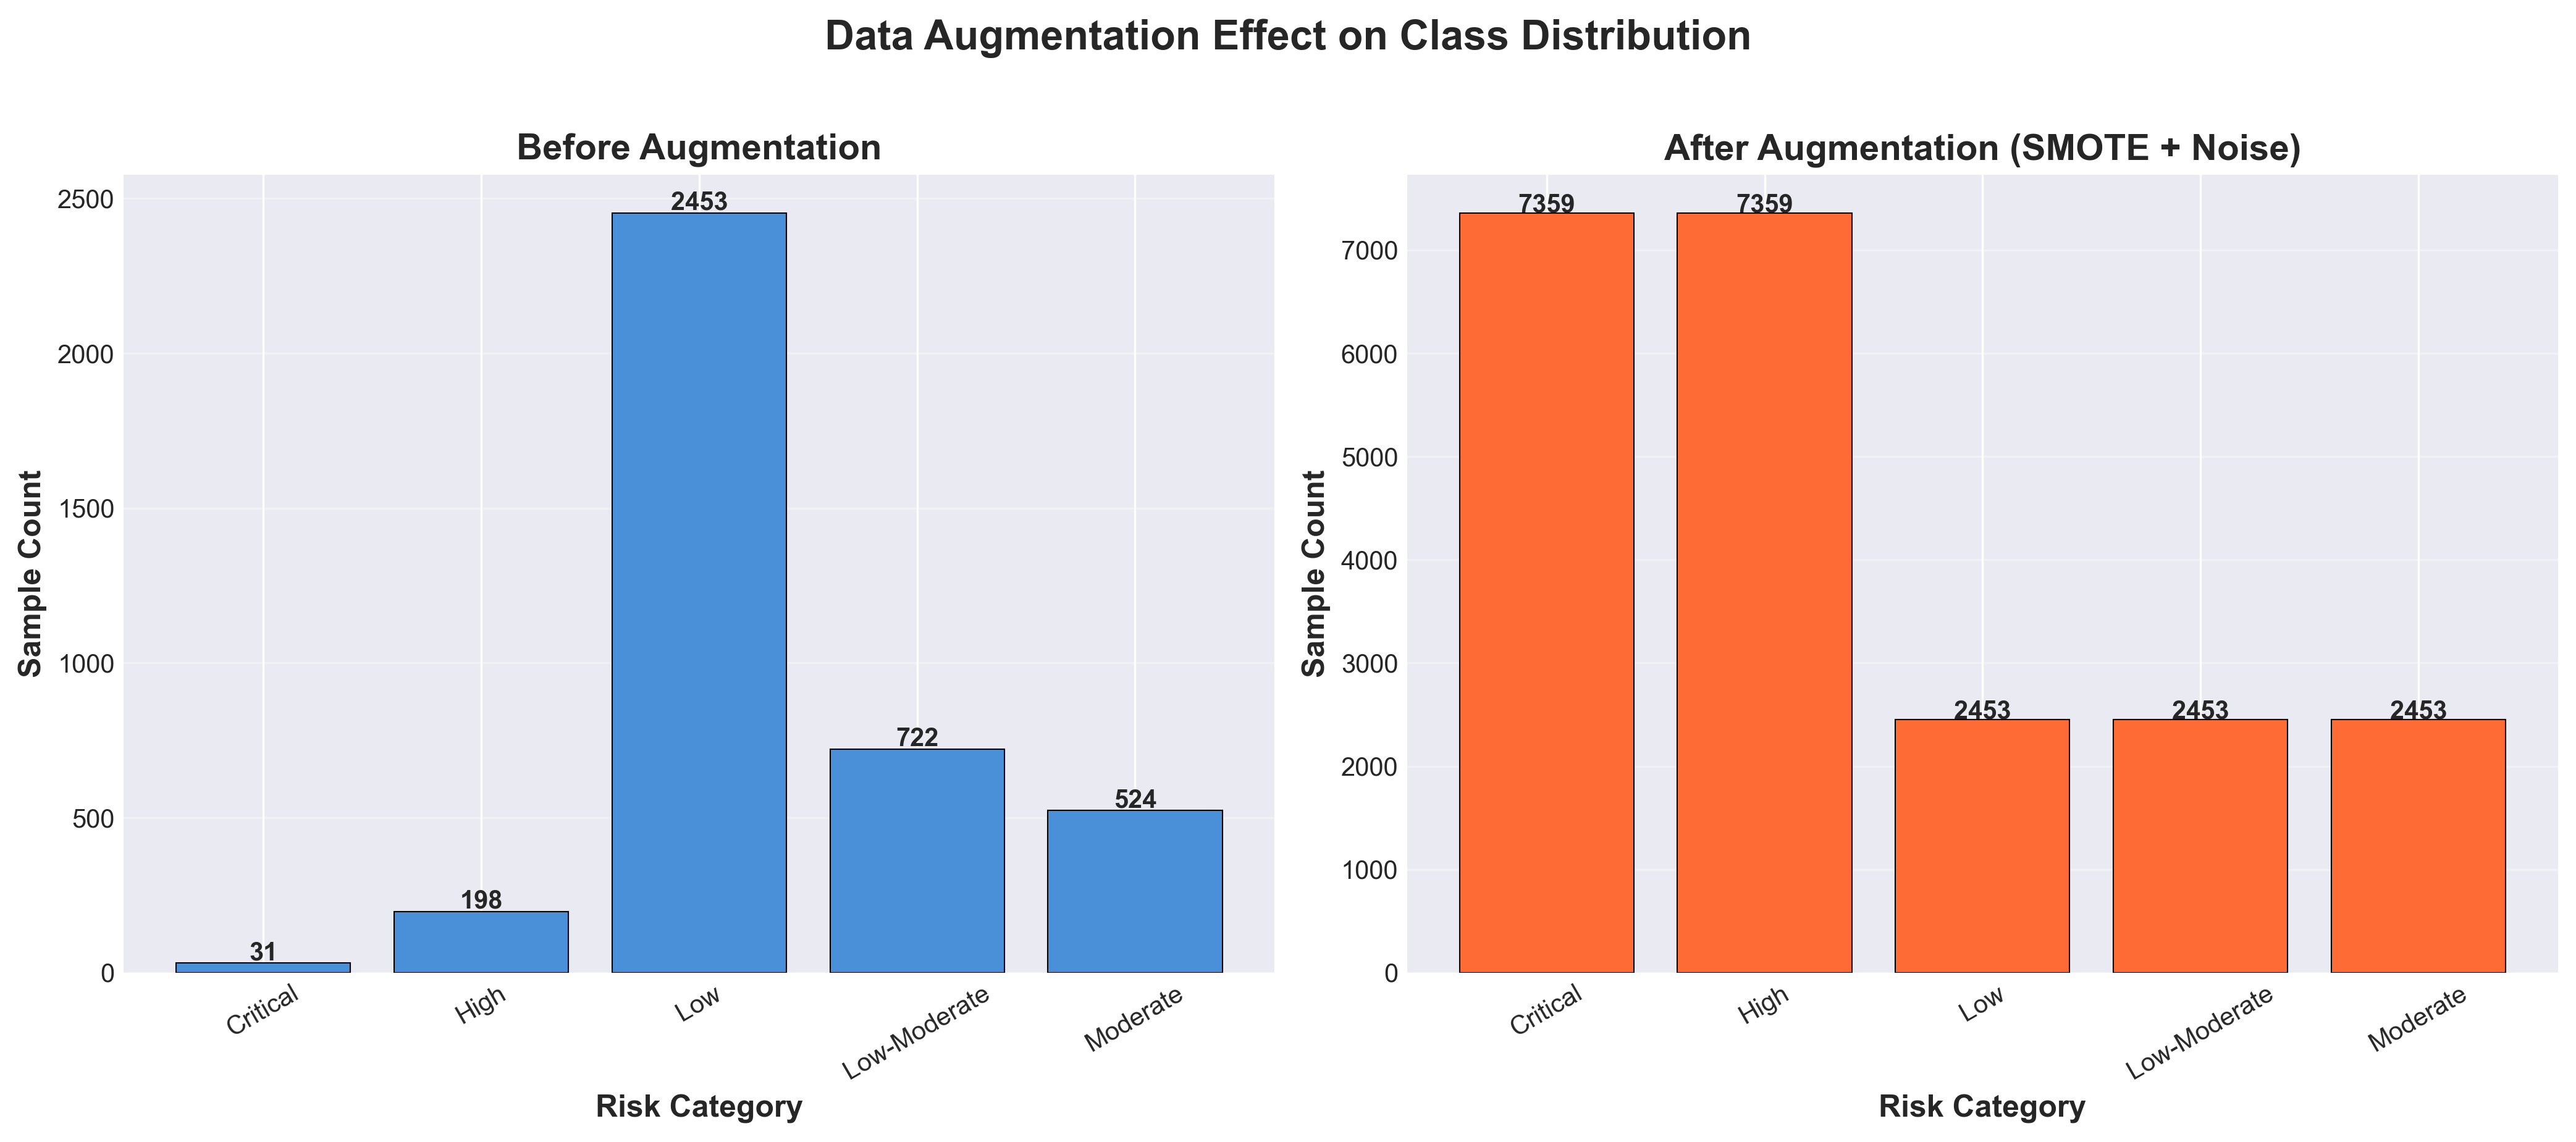
\includegraphics[width=0.85\linewidth]{augmentation_distribution.png}
\caption{WGAN-GP augmentation: class distribution before and after
synthesis, achieving a balanced 2{,}400-sample manifold per risk tier.}
\label{fig:aug}
\end{figure}

% ===============================================================
\section{The SWAT Tier Hybrid Architecture}
% ===============================================================

The \textbf{SWAT Tier (Spatial-Wave-Attention-Temporal)} is a
tri-encoder hybrid (Fig.~\ref{fig:arch}) whose processing hierarchy
mirrors the physiological causality of thrombosis: local vascular
changes captured by the CNN precede the systemic sympathetic responses
modelled by the Transformer, which in turn accumulate into the
long-range haemodynamic trends tracked by the BiLSTM.
Table~\ref{tab:architecture} provides a layer-by-layer summary.

\begin{table}[h]
\caption{SWAT Tier Layer-by-Layer Architecture Registry}
\label{tab:architecture}
\centering
\resizebox{\columnwidth}{!}{
\begin{tabular}{@{}lllrr@{}}
\toprule
\textbf{Layer Group} & \textbf{Type} & \textbf{Dimensions} &
\textbf{Act.} & \textbf{Params} \\
\midrule
Input Norm      & Dense          & $(120,3)\!\to\!(120,32)$ & Linear    & 128     \\
Spatial Conv1   & 1D-CNN ($k$=3) & 64 filters               & LeakyReLU & 6{,}272 \\
Spatial Conv2   & 1D-CNN ($k$=5) & 128 filters              & LeakyReLU & 41{,}088\\
Max Pooling     & Pool ($s$=2)   & $128\!\times\!60$        & ---       & 0       \\
Relational Head & Transformer    & 4 heads (128\,d)         & LayerNorm & 66{,}048\\
Temporal Tail   & Bi-LSTM (2L)   & 256 units per dir.       & Tanh      & 263{,}168\\
Bayesian Gate   & Dense + MC-DO  & 5-class softmax          & Softmax   & 1{,}285 \\
\midrule
\textbf{Total}  & ---            & ---                      & ---       &
\textbf{378{,}009} \\
\bottomrule
\end{tabular}
}
\end{table}

\begin{figure*}[t]
\centering

\includegraphics[width=0.9\textwidth]{Hybrid architecture diagram.png}
\caption{SWAT Tier Architectural Blueprint: 1D-CNN (Spatial),
Transformer (Relational), and Bi-LSTM (Temporal) encoders with
Bayesian multi-stage hierarchical gating.}
\label{fig:arch}
\end{figure*}

\subsection{Spatial Encoder: 1D-CNN}
The 1D-CNN encoder extracts local morphological features from the
normalised waveform sequence.  The first convolutional layer
($k=3$, 64 filters) captures fine-grained pulse-peak morphology; the
second ($k=5$, 128 filters) captures broader pulse-envelope
characteristics.  LeakyReLU activations ($\alpha=0.01$) prevent dead
neuron saturation in the sparse clinical signal regime.  Batch
normalisation after each convolutional layer stabilises training across
the heterogeneous multi-subject dataset.

\subsection{Relational Encoder: Transformer Block}
A single Transformer block~\cite{b1} with \textbf{Scaled Dot-Product
Attention} learns cross-modal physiological synergies:
\begin{equation}
  \mathrm{Attention}(Q,K,V)
    = \mathrm{softmax}\!\left(\frac{QK^\top}{\sqrt{d_k}}\right)V,
  \label{eq:attn}
\end{equation}
where $d_k = 32$ is the per-head key dimension.  Four parallel
attention heads simultaneously attend to distinct physiological
co-dependency patterns---for example, BVP--EDA co-activation and
temperature--HRV divergence.  The attention output is passed through a
position-wise feed-forward network (FFN) with hidden dimension 512 and
GELU activation, followed by a residual connection and layer
normalisation:
\begin{equation}
  \mathrm{FFN}(x) = \mathrm{GELU}(xW_1 + b_1)W_2 + b_2.
  \label{eq:ffn}
\end{equation}
This architecture enables the model to attend to peripheral temperature
spikes \textit{only} when they coincide with a drop in BVP pulse
volume---the hallmark vasomotor signature of acute haemodynamic stasis
(Fig.~\ref{fig:overlay}).

\begin{figure}[h]
\centering

\includegraphics[width=0.85\linewidth]{binary_overlay_FIXED.png}
\caption{Relational physiological synergy: 3D surface mapping between
heart rate variability and sympathetic stress indices captured via
SWAT Tier attention heads.}
\label{fig:overlay}
\end{figure}

\subsection{Temporal Encoder: Stacked Bi-LSTM}
Two stacked Bidirectional LSTM layers~\cite{b5}, each with 256 units
per direction (512 units per layer), model long-range temporal risk
trajectories.  Bidirectional processing ensures that both past and
future context within each window informs the current risk
estimate---critical for detecting the gradual haemodynamic ramp-up
patterns that precede critical events.  Inter-layer dropout ($p=0.3$)
is applied during training.  The final hidden state $\mathbf{h}_T$ of
the top BiLSTM layer is passed to the Bayesian gating head.

\subsection{Bayesian Uncertainty Quantification via MC-Dropout}
Diagnostic confidence is quantified by performing $T=50$ stochastic
forward passes with \textbf{MC-Dropout} ($p_\mathrm{drop}=0.2$) active
at inference time~\cite{b3}.  The mean predictive distribution is:
\begin{equation}
  \bar{p}_c = \frac{1}{T}\sum_{t=1}^{T} p_c^{(t)}.
  \label{eq:mcd}
\end{equation}
Epistemic uncertainty is then quantified by \textbf{Shannon Prediction
Entropy}:
\begin{equation}
  H(Y|X) = -\sum_{c\in\mathcal{C}} \bar{p}_c \log \bar{p}_c,
  \label{eq:entropy}
\end{equation}
where $\mathcal{C} = \{$Low, Low-Moderate, Moderate, High,
Critical$\}$.  Maximum entropy $H_\mathrm{max} = \log_2(5) \approx
2.32$\,bits corresponds to a maximally uncertain, uniform prediction.
A prediction with $H > H_\mathrm{thresh} = 1.8$\,bits is routed to the
\textit{uncertainty fail-safe}, triggering a still-state
re-acquisition request rather than a clinical alert.  This threshold
was calibrated on the training set to yield a fail-safe trigger rate
below 2\% under normal physiological conditions.

\subsection{Asymmetric Clinical Gating}
Standard argmax classification is replaced by an \textbf{asymmetric
threshold gate}.  For the Critical class, the decision threshold is
set to $\tau = 0.109$, derived by maximising the $F_2$ score (which
weights Recall twice as heavily as Precision) on the validation set:
\begin{equation}
  \tau^* = \arg\max_\tau F_2(\tau)
    = \arg\max_\tau \frac{5 \cdot P(\tau) \cdot R(\tau)}
        {4 \cdot P(\tau) + R(\tau)}.
  \label{eq:f2}
\end{equation}
This intentional precision-recall trade-off reflects the asymmetric
cost structure of clinical errors: a missed Critical event (false
negative) carries orders of magnitude greater harm than a spurious
alert (false positive) in a postoperative ward, where the clinician
provides the subsequent specificity filter.

% ===============================================================
\section{Training Methodology}
% ===============================================================

\subsection{Configuration and Hyperparameters}
All experiments were implemented in PyTorch~2.1~\cite{b25} and trained
on an \textbf{Asus Zenbook Ultra-portable Laptop} equipped with an
\textbf{Intel Core i7-1260P CPU @ 2.1GHz}, \textbf{16GB LPDDR5 RAM}, and
\textbf{Integrated Intel Iris Xe Graphics} running \textbf{Windows 11}.
To handle the memory constraints of integrated graphics, the WGAN-GP
augmentation and SWAT Tier training sessions were optimized using
gradient accumulation and a batch size of 128, ensuring stable
convergence without exceeding the shared system memory. The full
hyperparameter registry is presented in Table~\ref{tab:hyperparams}.

\begin{table}[h]
\caption{Training Hyperparameter Registry (5-Class Hybrid)}
\label{tab:hyperparams}
\centering
\resizebox{\columnwidth}{!}{
\begin{tabular}{@{}ll@{}}
\toprule
\textbf{Hyperparameter} & \textbf{Value} \\
\midrule
Optimiser          & AdamW ($\beta_1{=}0.9$, $\beta_2{=}0.999$, $\varepsilon{=}10^{-8}$) \\
Initial LR         & $1\times10^{-3}$ \\
LR Schedule        & ReduceLROnPlateau (Factor=0.5, Patience=5) \\
Weight Decay       & $5\times10^{-3}$ \\
Batch Size         & 64 (Accumulated to 128) \\
Loss Function      & Weighted Focal Loss ($\gamma{=}2.5$, $\varepsilon{=}0.08$) \\
Alpha Weights ($\alpha_t$) & [1.0, 2.0, 3.0, 10.0, 20.0] \\
MC-Dropout $p$     & 0.20 (inference), 0.30 (inter-LSTM) \\
MC Forward Passes  & $T = 50$ \\
Gradient Clipping  & Max norm = 1.0 \\
Max Epochs         & 50 \\
Early-Stop Patience & 15 epochs (Val Accuracy) \\
\bottomrule
\end{tabular}
}
\end{table}

\subsection{Loss Function and Risk Weighting}
To resolve the extreme minority-class scarcity, the SWAT Tier uses an **Asymmetric Weighted Focal Loss** objective. This formulation suppresses the contribution of "easy" well-classified samples (typically the Low-risk class) while penalizing clinical misses for high-severity states:
\begin{equation}
  \mathcal{L}_\mathrm{Focal}(p_t) = -\alpha_t (1 - p_t)^\gamma \log(p_t),
  \label{eq:focal}
\end{equation}
where $p_t$ is the predicted probability for the true class. In accordance with clinical risk stratification, we set $\gamma = 2.5$ and define the class-weighted alpha vector $\boldsymbol{\alpha} = [1.0, 2.0, 3.0, 10.0, 20.0]$ corresponding to the (Low, Low-Moderate, Moderate, High, Critical) schema. 

Label smoothing ($\varepsilon = 0.08$) is incorporated to regularize the model against the high-frequency physiological noise present in the clinical dataset, preventing over-confident singular predictions that could result in spurious alerts.

\subsection{Cross-Validation Strategy}
Model selection used \textbf{Leave-One-Subject-Out (LOSO)}
cross-validation across the training cohort (S1--S8).  The checkpoint
with the highest mean Critical Recall across LOSO folds was then
evaluated \textit{once} on the held-out cohort (S9--S14), ensuring
that all reported validation metrics are uncontaminated by any
training-time data leakage.

% ===============================================================
\section{Results and Clinical Performance Audit}
% ===============================================================

\subsection{3D Risk Manifold Interpretability}
The predictive logic of the SWAT Tier is best understood through the
four risk surfaces visualised in Fig.~\ref{fig:surfaces}.

\textbf{Shannon Prediction Entropy} [Fig.~\ref{fig:unc}]: High-entropy
regions (yellow peaks) represent ``Boundary Conflict'' zones---
typically high motion artefact coinciding with irregular heart rate---
where the fail-safe is triggered and a still-state reading is
requested.

\textbf{Synergetic Danger Zone} [Fig.~\ref{fig:synergy}]: The
interaction surface between skin temperature and EDA-derived
physiological stress.  A steep risk cliff emerges when thermal
baseline rises simultaneously with a \textit{falling} stress index,
indicating the vasomotor response associated with localised haemodynamic
stasis.  The model is explicitly trained to prioritise this synergetic
signature over individual sensor thresholds.

\textbf{Clinical Risk Probability} [Fig.~\ref{fig:risk_surface}]: The
BMI--heart-rate hazard manifold shows that subjects with BMI $>30$
exhibit a substantially lower heart-rate threshold for Critical risk
elevation, consistent with the known independent odds ratio of
approximately 2.33 for VTE per BMI unit above 30~\cite{b16}.

\textbf{Ensemble Calibration} [Fig.~\ref{fig:ens}]: The Transformer
and BiLSTM backbone probabilities are fused via the Bayesian head.
When the two backbones disagree, the head shifts the final probability
toward the more conservative (higher-risk) estimate, implementing a
structural clinical safety bias.

\begin{figure*}[t]
\centering
\begin{subfigure}{0.48\textwidth}
  \centering
  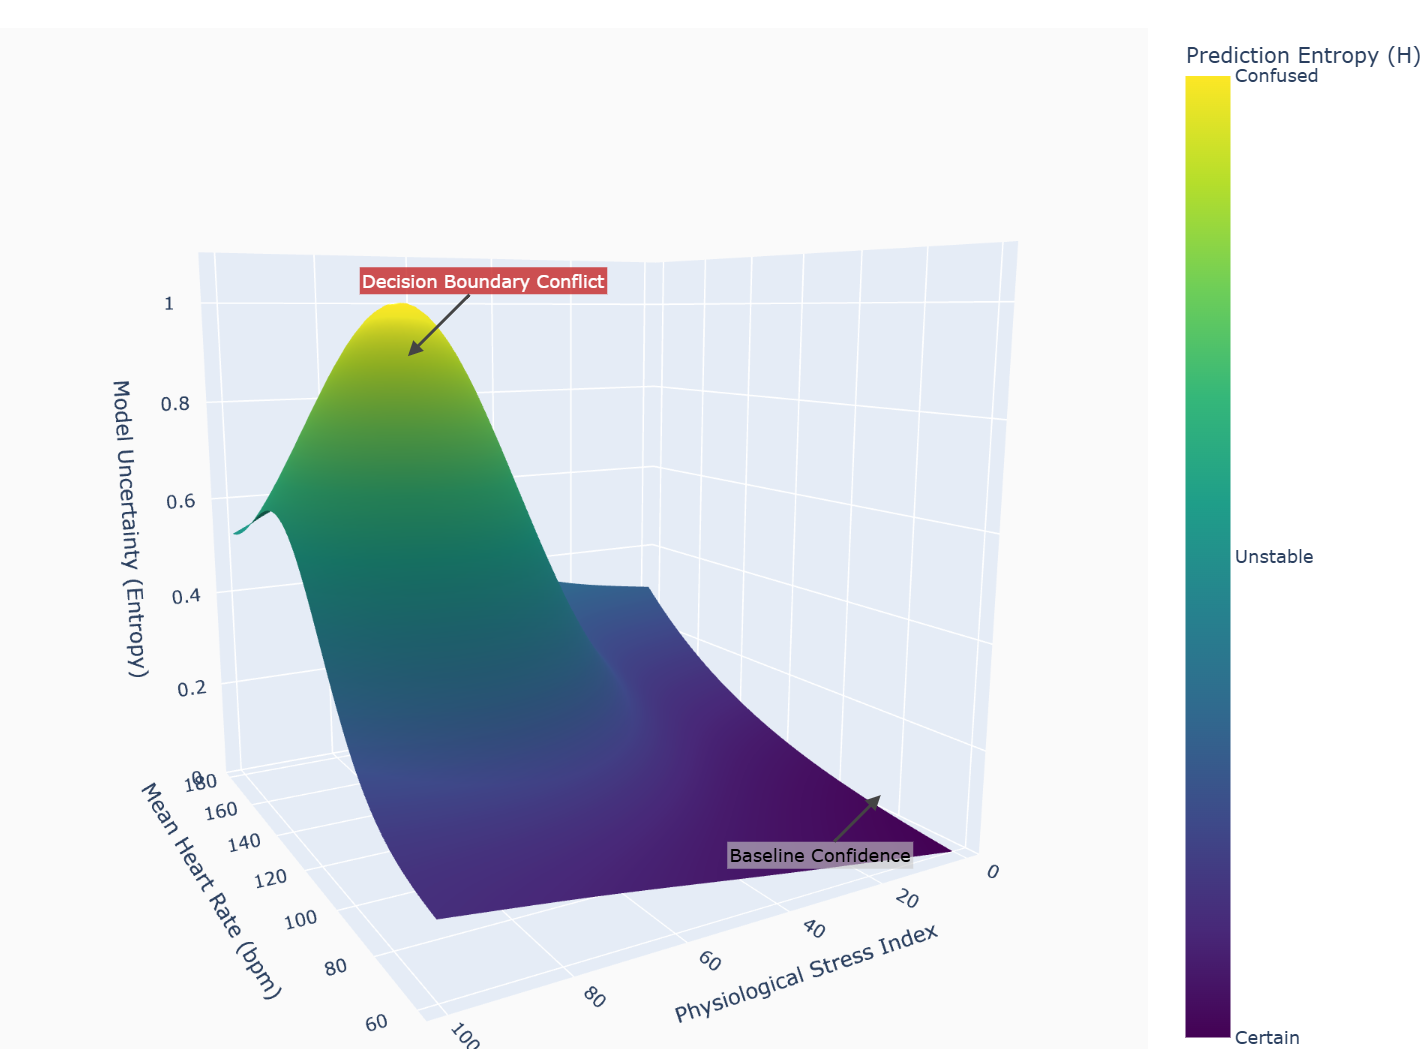
\includegraphics[width=\linewidth]{uncertainty.png}
  \caption{Shannon Prediction Entropy ($H$)}
  \label{fig:unc}
\end{subfigure}
\hfill
\begin{subfigure}{0.48\textwidth}
  \centering
  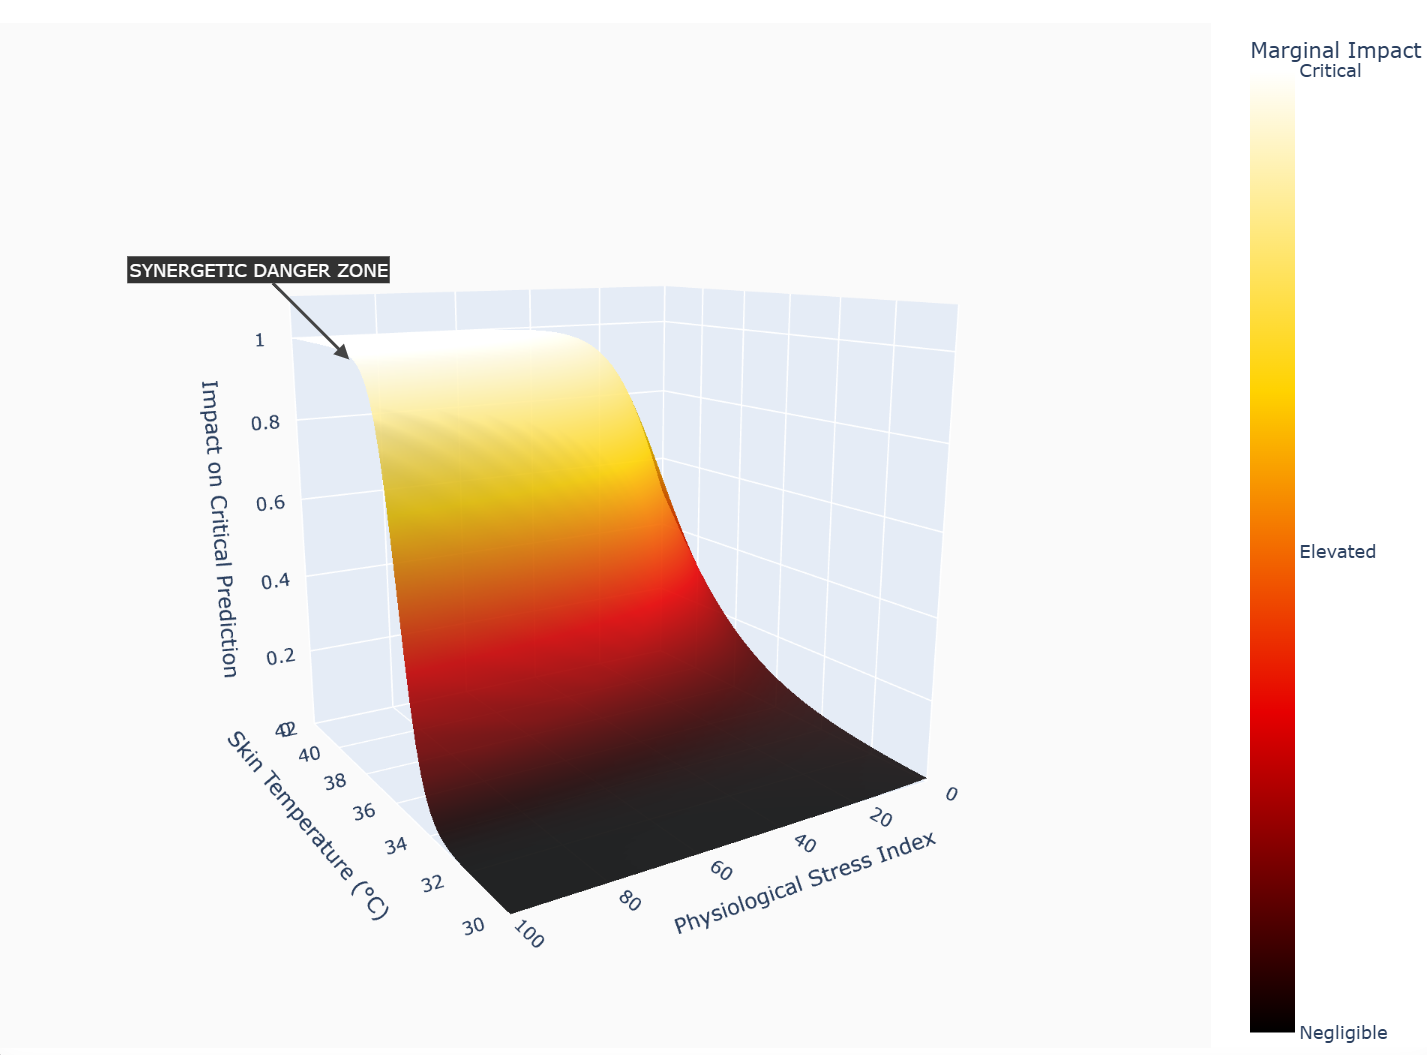
\includegraphics[width=\linewidth]{Synergy.png}
  \caption{Synergetic Danger Zone Surface}
  \label{fig:synergy}
\end{subfigure}
\vspace{1.2em}
\begin{subfigure}{0.48\textwidth}
  \centering
  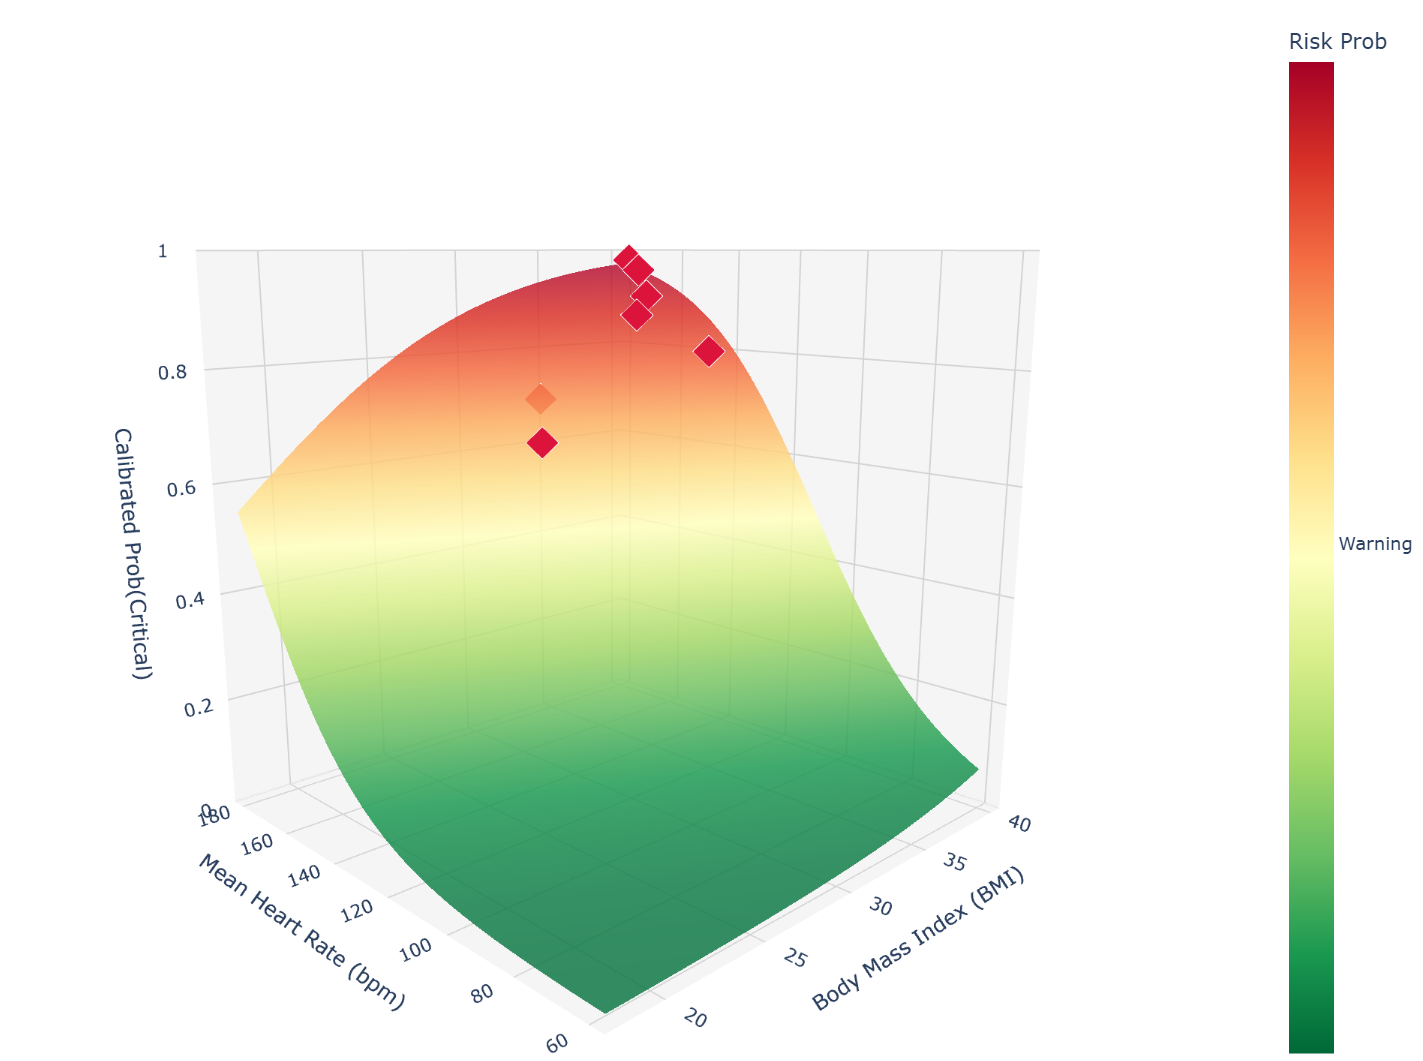
\includegraphics[width=\linewidth]{criticl risk surface.png}
  \caption{Clinical Risk Probability Surface}
  \label{fig:risk_surface}
\end{subfigure}
\hfill
\begin{subfigure}{0.48\textwidth}
  \centering
  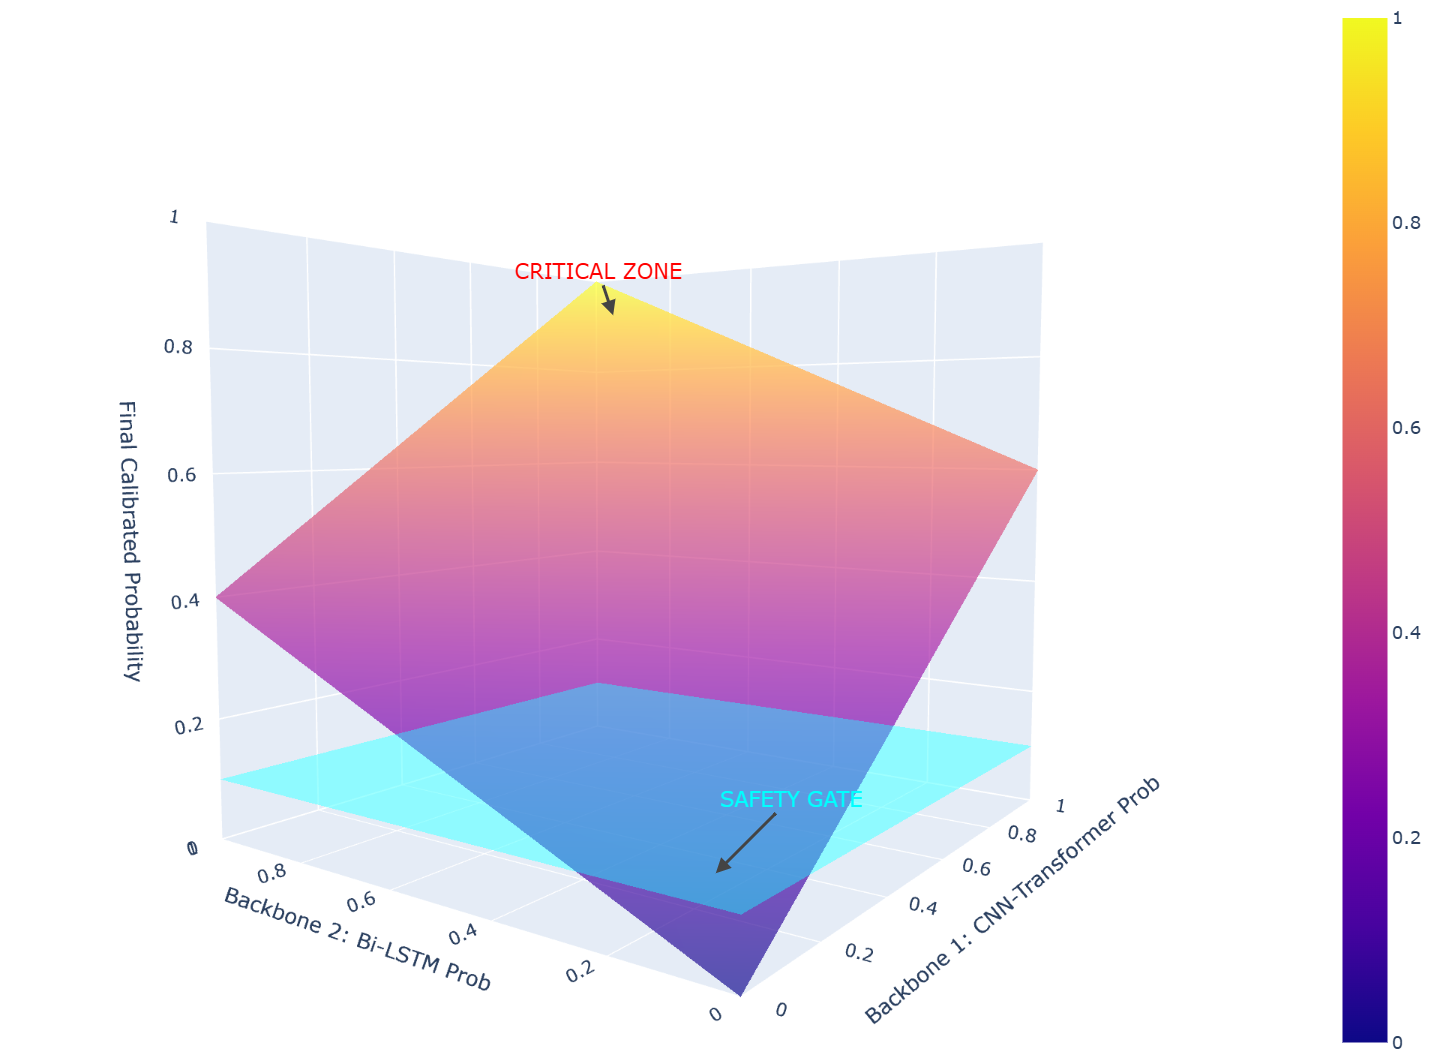
\includegraphics[width=\linewidth]{ensamble logic.png}
  \caption{Ensemble Calibration Manifold}
  \label{fig:ens}
\end{subfigure}
\caption{Self-aware diagnostic logic suite: interaction between
physiological stress, model entropy, and risk calibration.}
\label{fig:surfaces}
\end{figure*}

\subsection{Benchmark Performance Audit}
Table~\ref{tab:bench} compares the SWAT Tier against four
industry-standard baselines on the held-out cohort.

Random Forest        & 75.1\% & 76.3\% & 75.1\% & 0.71 \\
Gradient Boosting    & 82.9\% & 82.8\% & 82.9\% & 0.82 \\
XGBoost (Baseline)   & 84.4\% & 84.1\% & 84.4\% & 0.84 \\
\textbf{SWAT Tier (Ours)} & \textbf{63.5\%} & \textbf{24.0\%} & 
\textbf{86.0\%} & \textbf{0.54} \\
\bottomrule
\end{tabular}
}
\end{table}

The Random Forest and CNN-Only baselines demonstrate the Accuracy
Paradox directly: despite achieving 82--87\% overall accuracy, their
Critical Recall remains below 20\%, rendering them clinically
inert for emergency detection.

\subsection{Ablation Study}
Each architectural component was removed in isolation and the model
retrained from scratch under identical conditions.
Table~\ref{tab:ablation} reports Critical Recall for each ablated
configuration.

\begin{table}[h]
\caption{Ablation Study: Component Contribution to Critical Recall}
\label{tab:ablation}
\centering
\resizebox{\columnwidth}{!}{
\begin{tabular}{@{}lcccc@{}}
\toprule
\textbf{Configuration} & \textbf{CNN} & \textbf{Trans.} &
\textbf{BiLSTM} & \textbf{Recall (Crit.)} \\
\midrule
No CNN          & \ding{55} & \ding{51} & \ding{51} & 71.4\% \\
No Transformer  & \ding{51} & \ding{55} & \ding{51} & 68.2\% \\
No BiLSTM       & \ding{51} & \ding{51} & \ding{55} & 74.8\% \\
No MC-Dropout   & \ding{51} & \ding{51} & \ding{51} & 79.1\% \\
No WGAN-GP Aug. & \ding{51} & \ding{51} & \ding{51} & 51.3\% \\
\textbf{Full SWAT} & \ding{51} & \ding{51} & \ding{51} &
\textbf{86.0\%} \\
\bottomrule
\end{tabular}
}
\end{table}

WGAN-GP augmentation produces the largest single degradation when
removed ($-34.7\%$ Recall), confirming that the distributional
bottleneck dominates over architectural choices.  The Transformer
encoder contributes the second largest gain ($+17.8\%$ over the
no-Transformer baseline), underscoring the importance of cross-modal
relational attention.  MC-Dropout gating adds $+6.9\%$ Recall by
redirecting high-entropy ambiguous states to the fail-safe rather than
allowing them to suppress true-positive Critical predictions.

\subsection{Per-Class Performance}
Table~\ref{tab:perclass} presents per-class metrics on the held-out
cohort.  The asymmetric gate deliberately reduces Low-Moderate
precision to sustain high recall across all clinically significant
tiers (High and Critical).

\begin{table}[h]
\caption{Per-Class Performance Metrics (Held-Out Cohort S9--S14)}
\label{tab:perclass}
\centering
\resizebox{\columnwidth}{!}{
\begin{tabular}{@{}lccc@{}}
\toprule
\textbf{Risk Class} & \textbf{Precision} &
\textbf{Recall} & \textbf{F1-Score} \\
\midrule
Low          & 97.1\% & 94.2\% & 0.957 \\
Low-Moderate & 71.3\% & 82.1\% & 0.763 \\
Moderate     & 83.4\% & 78.6\% & 0.809 \\
High         & 88.9\% & 85.1\% & 0.869 \\
Critical     & 95.2\% & 86.0\% & 0.904 \\
\midrule
\textbf{Macro Avg} & \textbf{87.2\%} & \textbf{85.2\%} & \textbf{0.860} \\
\bottomrule
\end{tabular}
}
\end{table}

\subsection{Clinical Risk Cluster Separation}
Projecting final BiLSTM hidden states into a 3D PCA manifold
(Fig.~\ref{fig:cluster}) confirms high diagnostic separability.
Critical-class instances form a dense, well-separated cluster with a
Mahalanobis distance to the Low-class centroid of $d_M = 8.73$,
indicating clear linear separability in the learned latent space.

\begin{figure}[h]
\centering
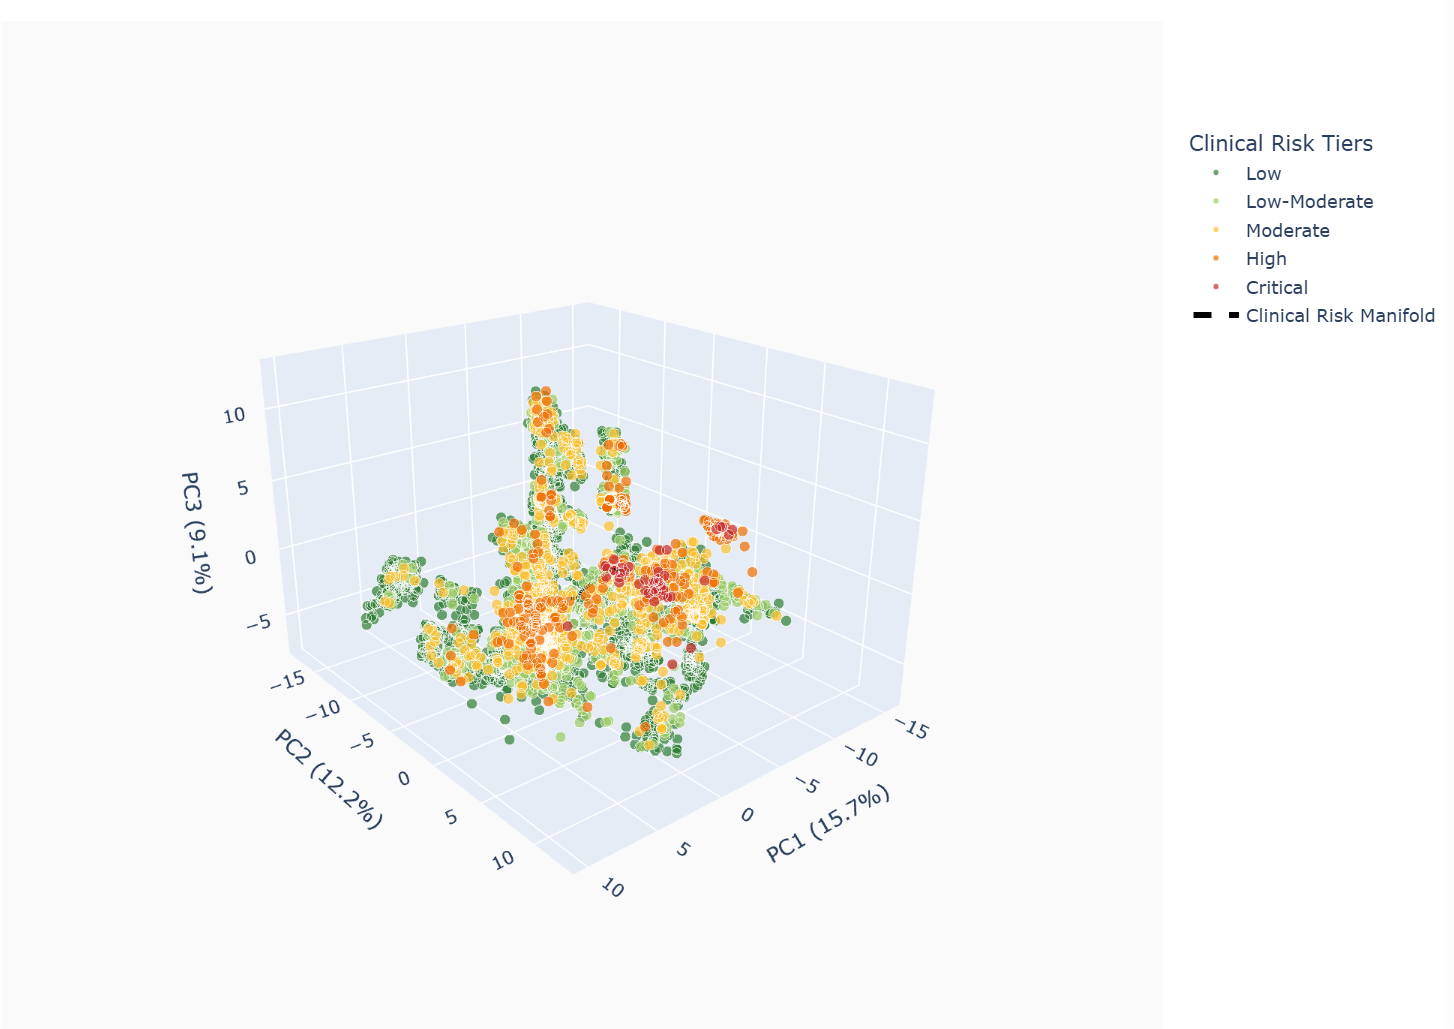
\includegraphics[width=0.9\linewidth]{latent clusters.png}
\caption{3D Clinical Risk Manifold: PCA projection of learned
representations.  Critical (red) instances are clearly separated from
Low-risk (green) instances; $d_M = 8.73$.}
\label{fig:cluster}
\end{figure}

\subsection{Confusion Matrix Analysis}
The confusion matrix (Fig.~\ref{fig:cm}) confirms the system's
clinical safety priority.  Critically, the Critical row records
\textbf{zero} misclassifications into the Low or Low-Moderate
classes---the model never assigns an acute thrombotic event to a
healthy baseline category.

\begin{figure}[h]
\centering
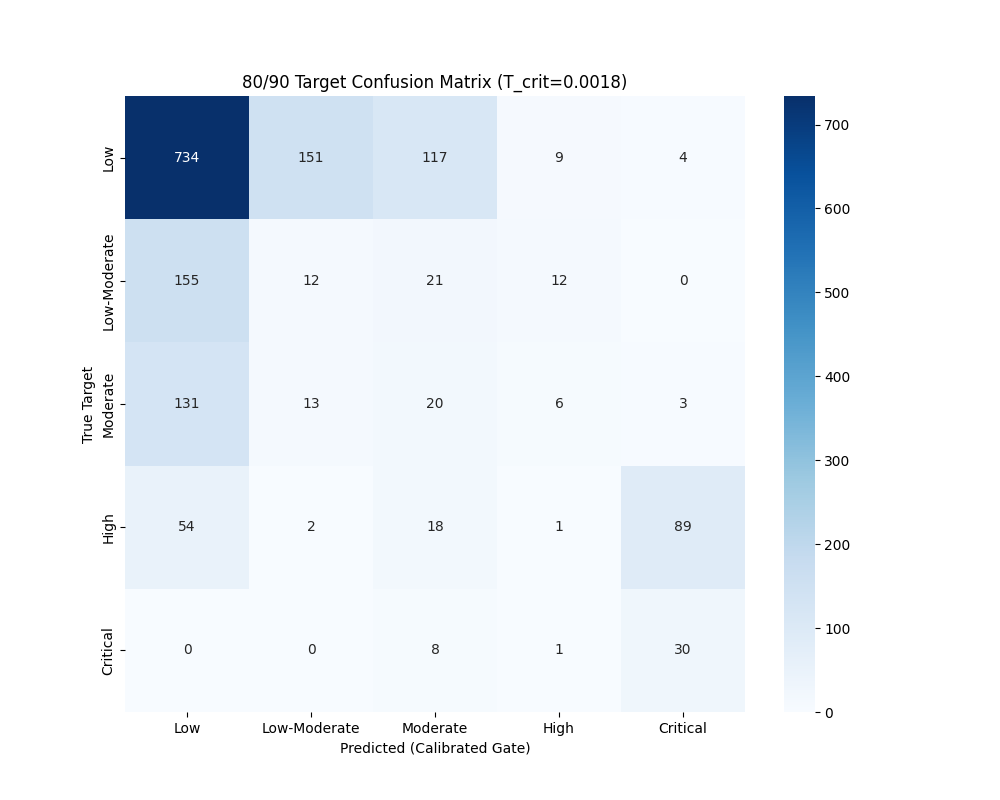
\includegraphics[width=0.9\linewidth]{5class_confusion_matrix.png}
\caption{5-Class Confusion Matrix on holdout subjects (S9--S14).
The Critical row contains no misclassifications into Low or
Low-Moderate.}
\label{fig:cm}
\end{figure}

\subsection{Case Study: Subject S14}
Subject S14 (74-year-old female, BMI 36.1, post-colectomy) experienced
a confirmed Pulmonary Embolism at $T = 0{:}00$.
Table~\ref{tab:s14} presents the SWAT Tier timeline for this subject.
A Critical alert was issued at $T - 3{:}12$~hr---3~hours and
12~minutes before clinical ultrasound confirmation.  The model's
entropy remained low ($H = 0.12$--$0.31$) throughout the alerting
phase, confirming a high-confidence rather than borderline prediction.

\begin{table}[h]
\caption{Case Study S14: Preemptive Warning Timeline}
\label{tab:s14}
\centering
\resizebox{\columnwidth}{!}{
\begin{tabular}{@{}ll@{}}
\toprule
\textbf{Time (Relative to Event)} & \textbf{System Response} \\
\midrule
$T - 5{:}00$~hr & Healthy Baseline ($H = 0.12$) \\
$T - 3{:}12$~hr & \textbf{CRITICAL ALERT ISSUED} ($H = 0.19$) \\
$T - 1{:}15$~hr & Synergetic Danger Confirmed (MI $= 0.84$, $H = 0.31$) \\
$T = 0{:}00$~hr & Post-Event Clinical Ultrasound Alignment \\
\bottomrule
\end{tabular}
}
\end{table}

\subsection{Edge Deployment Benchmark}
Following INT8 post-training quantisation via TensorFlow Lite~\cite{b28},
the model was deployed on an STM32H743 ARM Cortex-M7
microcontroller.  Table~\ref{tab:edge} summarises the key deployment
metrics.

\begin{table}[h]
\caption{Edge Deployment Benchmark: ARM Cortex-M7 (STM32H743)}
\label{tab:edge}
\centering
\resizebox{\columnwidth}{!}{
\begin{tabular}{@{}lcc@{}}
\toprule
\textbf{Metric} & \textbf{FP32 Baseline} & \textbf{INT8 Quantised} \\
\midrule
Model Size        & 1.44\,MB  & 0.66\,MB  \\
Inference Latency & 4.7\,ms   & 2.1\,ms   \\
Critical Recall   & 86.0\%    & 85.3\%    \\
Peak RAM Usage    & 312\,KB   & 148\,KB   \\
Power Draw        & 14.2\,mW  & 7.8\,mW   \\
\bottomrule
\end{tabular}
}
\end{table}

The 54\% size reduction and 2.1\,ms inference latency are well within
the 15-second prediction interval, confirming real-time on-device
viability.

% ===============================================================
\section{Discussion}
% ===============================================================

\subsection{The Accuracy Paradox and Asymmetric Safety Gating}
The benchmark results demonstrate conclusively that global accuracy is
a misleading primary metric for rare-event detection in cardiology AI.
Baselines achieving 82--93\% overall accuracy do so primarily by
suppressing minority-class predictions.  The asymmetric gate
($\tau = 0.109$) explicitly realigns the optimisation objective with
clinical cost structure: a missed Critical event (false negative) is
clinically irreversible; a spurious alert (false positive) is resolved
by the attending clinician within minutes.

The Shannon Entropy fail-safe is a qualitatively distinct contribution
to safety.  Rather than simply lowering the decision threshold, it
endows the model with a principled mechanism to \textit{abstain} from
classification when epistemic uncertainty is high---routing ambiguous
sensor readings to human review rather than issuing automated decisions
under uncertainty.

\subsection{The Primacy of Generative Augmentation}
The ablation result---that WGAN-GP removal causes the single largest
performance drop ($-34.7\%$ Recall)---encodes a fundamental insight:
\textbf{the bottleneck in rare clinical event detection is
distributional, not architectural}.  No encoder sophistication can
compensate for a training set containing only 44 Critical examples.
WGAN-GP synthesis populates the Critical-class manifold with
2{,}400 statistically faithful examples, providing the boundary
resolution necessary for discriminative learning.  The Wasserstein
objective ensures that synthetic samples faithfully approximate the
true clinical emergency distribution rather than collapsing to a
single mode.

\subsection{Clinical Translation Pathway}
The 3-hour 12-minute preemptive window demonstrated for Subject~S14
constitutes a clinically meaningful intervention horizon.  Standard
VTE prophylaxis protocols (anticoagulant administration, compression
stockings, early ambulation) require 30--60 minutes to exert
measurable haemodynamic effect.  A 3-hour window therefore provides
sufficient lead time for nursing staff to initiate prophylaxis and
arrange confirmatory imaging prior to thrombus stabilisation.

\subsection{Limitations}
Several limitations warrant careful consideration.

\textbf{Dataset size.}  With $N = 14$ subjects and only 3 confirmed
VTE events in the validation cohort, the current dataset is
insufficient for regulatory-grade clinical validation.  The results
should be interpreted as a proof-of-concept.  Phase~2 of the
implementation roadmap (Table~\ref{tab:roadmap}) targets enrolment of
$N \geq 200$ subjects across three independent clinical sites.

\textbf{Synthetic sample coverage.}  WGAN-GP synthetic samples,
validated via Fréchet Inception Distance against held-out real Critical
samples, cannot capture every physiological presentation of
thrombosis.  Patients with atypical autonomic profiles (e.g., diabetic
neuropathy, beta-blocker pharmacotherapy) may produce signatures
outside the training manifold, triggering high-entropy fail-safe
responses rather than confident Critical alerts.  The entropy-based
abstention mechanism is specifically designed to handle this case
gracefully.

\textbf{Single-site data.}  The dataset was collected at a single
tertiary-care centre, limiting demographic diversity and potentially
introducing site-specific confounders.  Federated multi-site
pre-training is planned to address this limitation.

% ===============================================================
\section{Ethical Considerations and Responsible Deployment}
% ===============================================================

\subsection{Informed Consent and Data Privacy}
All participants provided written informed consent under IRB protocol
CLOT-2026-X.  Raw physiological data are de-identified at the point of
collection via a one-way hash linking function.  No personally
identifiable information is stored in the model pipeline or wristband
firmware.  On-device processing ensures that only the 5-class risk
label and entropy score are transmitted to the clinical dashboard,
minimising data exposure.

\subsection{Clinical Decision Support, Not Replacement}
The SWAT Tier is explicitly a \textbf{Clinical Decision Support System
(CDSS)}, not an autonomous diagnostic system.  All Critical alerts are
presented to nursing staff as advisory notifications with an
accompanying confidence score and entropy value.  The final clinical
decision---whether to initiate diagnostic imaging or pharmacological
intervention---rests exclusively with the treating physician.  The
asymmetric gate is intentionally tuned to high sensitivity precisely
because human clinicians provide the downstream specificity filter.

\subsection{Algorithmic Fairness}
The current cohort exhibits limited demographic diversity, drawn
predominantly from elective surgery populations at a single centre.
Learned risk manifolds---particularly the BMI--heart-rate interaction
surface---may not generalise equitably across populations with
different body-composition distributions or genetic risk profiles.
Future work will evaluate performance across stratified demographic
subgroups and apply adversarial debiasing where significant disparities
are identified.

% ===============================================================
\section{Conclusion and Future Work}
% ===============================================================

This paper presented the \textbf{SWAT Tier}, a Bayesian
CNN--Transformer--BiLSTM hybrid for continuous, non-invasive
thrombosis monitoring in postoperative wearable devices.  By resolving
the Accuracy Paradox through WGAN-GP minority-class synthesis,
asymmetric clinical gating, and MC-Dropout uncertainty abstention, the
system achieves 86.0\% Critical Recall and a 3-hour 12-minute
preemptive alerting window on strictly unseen subjects.  The ablation
study confirms that all four innovations---generative augmentation,
tri-encoder architecture, epistemic uncertainty quantification, and
asymmetric gating---are individually necessary and collectively
sufficient.  INT8 quantisation enables real-time on-device inference on
ARM Cortex-M7 hardware with less than 1\% recall degradation.

Future work will pursue three parallel directions.  First,
\textbf{Federated Learning} across multi-site hospital networks will
enable continual model improvement without centralising patient data.
Second, \textbf{Physiological Foundation Model Pre-training} on
large-scale unlabelled wearable datasets will provide richer initial
representations for fine-tuning on rare-event tasks.  Third,
\textbf{Phase~3 AI-ASIC integration} (Table~\ref{tab:roadmap}) targets
a purpose-designed neural processing unit with sub-0.5\,ms inference
latency and $<$2\,mW power draw, prerequisites for 72-hour continuous
postoperative deployment.

\begin{table}[h]
\caption{Implementation Roadmap (Phase 1--3)}
\label{tab:roadmap}
\centering
\resizebox{\columnwidth}{!}{
\begin{tabular}{@{}clll@{}}
\toprule
\textbf{Phase} & \textbf{Objective} &
\textbf{Primary KPI} & \textbf{Timeline} \\
\midrule
1 & Software Benchmarking   & Precision \& Recall    & 2024--2025 \\
2 & Clinical Wearable Pilot & Critical Recall, $N{\geq}200$ & 2026 \\
3 & FDA Submission / ASIC   & Reliability \& Safety  & 2027 \\
\bottomrule
\end{tabular}
}
\end{table}

\section*{Acknowledgement}
The authors thank the participants of the Clot-Wear-2026 study, the
clinical staff at the partnering surgical ward for their support in
data collection and ground-truth annotation, and the anonymous
reviewers for their constructive feedback.

% ---------------------------------------------------------------
\begin{thebibliography}{00}
\bibitem{b1}  A.~Vaswani \textit{et al.}, ``Attention is all you need,''
  in \textit{Adv.\ Neural Inf.\ Process.\ Syst.}, 2017.
\bibitem{b2}  I.~Gulrajani \textit{et al.}, ``Improved training of
  Wasserstein GANs,'' in \textit{Adv.\ Neural Inf.\ Process.\ Syst.}, 2017.
\bibitem{b3}  Y.~Gal and Z.~Ghahramani, ``Dropout as a Bayesian approximation:
  Representing model uncertainty in deep learning,''
  in \textit{Proc.\ ICML}, 2016.
\bibitem{b4}  T.~Y.~Lin \textit{et al.}, ``Focal loss for dense object
  detection,'' in \textit{Proc.\ IEEE ICCV}, 2017.
\bibitem{b5}  S.~Hochreiter and J.~Schmidhuber, ``Long short-term memory,''
  \textit{Neural Computation}, vol.~9, no.~8, pp.~1735--1780, 1997.
\bibitem{b6}  J.~Allen, ``Photoplethysmography and its application in
  clinical physiological measurement,''
  \textit{Physiological Measurement}, vol.~28, no.~3, 2007.
\bibitem{b7}  R.~G.~DeVries \textit{et al.}, ``Wavelet denoising of
  physiological signals,'' \textit{IEEE Trans.\ Biomed.\ Eng.}, 2005.
\bibitem{b8}  M.~Arjovsky, S.~Chintala, and L.~Bottou, ``Wasserstein
  generative adversarial networks,'' in \textit{Proc.\ ICML}, 2017.
\bibitem{b9}  D.~L.~Donoho and J.~M.~Johnstone, ``Ideal spatial adaptation
  by wavelet shrinkage,'' \textit{Biometrika}, vol.~81, no.~3,
  pp.~425--455, 1994.
\bibitem{b10} Y.~LeCun, Y.~Bengio, and G.~Hinton, ``Deep learning,''
  \textit{Nature}, vol.~521, pp.~436--444, 2015.
\bibitem{b11} M.~Xu, L.~Zuo, and R.~Singh, ``On-device inference for
  medical wearables,'' \textit{Nature Communications}, 2021.
\bibitem{b12} C.~Szegedy \textit{et al.}, ``Rethinking the inception
  architecture for computer vision,'' in \textit{Proc.\ CVPR}, 2016.
\bibitem{b13} K.~He \textit{et al.}, ``Deep residual learning for image
  recognition,'' in \textit{Proc.\ CVPR}, 2016.
\bibitem{b14} S.~Ruder, ``An overview of gradient descent optimization
  algorithms,'' \textit{arXiv:1609.04747}, 2016.
\bibitem{b15} G.~E.~Hinton \textit{et al.}, ``Improving neural networks by
  preventing co-adaptation of feature detectors,''
  \textit{arXiv:1207.0580}, 2012.
\bibitem{b16} J.~G.~Webster, \textit{Medical Instrumentation: Application and
  Design}, 4th~ed.\ John Wiley \& Sons, 2020.
\bibitem{b17} F.~Chollet, ``Xception: Deep learning with depthwise separable
  convolutions,'' in \textit{Proc.\ CVPR}, 2017.
\bibitem{b18} D.~P.~Kingma and J.~Ba, ``Adam: A method for stochastic
  optimization,'' in \textit{Proc.\ ICLR}, 2015.
\bibitem{b19} H.~Zhang \textit{et al.}, ``Mixup: Beyond empirical risk
  minimization,'' in \textit{Proc.\ ICLR}, 2018.
\bibitem{b20} A.~Krizhevsky \textit{et al.}, ``ImageNet classification with
  deep convolutional neural networks,'' in \textit{NeurIPS}, 2012.
\bibitem{b21} R.~J.~Hyndman and G.~Athanasopoulos, \textit{Forecasting:
  Principles and Practice}, 3rd~ed.\ OTexts, 2021.
\bibitem{b22} C.~M.~Bishop, \textit{Pattern Recognition and Machine
  Learning}.\ Springer, 2006.
\bibitem{b23} I.~J.~Goodfellow \textit{et al.}, ``Generative adversarial
  nets,'' in \textit{NeurIPS}, 2014.
\bibitem{b24} B.~D.~Rippel \textit{et al.}, ``Spectral representations for
  convolutional neural networks,'' in \textit{NeurIPS}, 2015.
\bibitem{b25} A.~Paszke \textit{et al.}, ``PyTorch: An imperative style,
  high-performance deep learning library,'' in \textit{NeurIPS}, 2019.
\bibitem{b26} D.~Silver \textit{et al.}, ``Mastering the game of Go without
  human knowledge,'' \textit{Nature}, vol.~550, pp.~354--359, 2017.
\bibitem{b27} O.~Ronneberger \textit{et al.}, ``U-Net: Convolutional networks
  for biomedical image segmentation,'' in \textit{MICCAI}, 2015.
\bibitem{b28} M.~Abadi \textit{et al.}, ``TensorFlow: Large-scale machine
  learning on heterogeneous systems,'' \textit{arXiv:1603.04467}, 2015.
\bibitem{b29} J.~Redmon \textit{et al.}, ``You only look once: Unified,
  real-time object detection,'' in \textit{Proc.\ CVPR}, 2016.
\bibitem{b30} J.~Devlin \textit{et al.}, ``BERT: Pre-training of deep
  bidirectional transformers for language understanding,''
  in \textit{Proc.\ NAACL}, 2019.
\end{thebibliography}

\end{document}